\section{Analisi funzionale}
Prima di iniziare lo sviluppo della piattaforma è necessario definire il framework sulla quale si appoggerà, in questo caso ho scelto il web framework ASP.NET Core che fa parte del framework general-purpose .NET 5.0 \cite{NET5.0}. Questo framework è stato sviluppato completamente da Microsoft ed offre numerosi vantaggi tra i quali il supporto cross-platform, la disponibilità del codice open-source in modo gratuito, costanti aggiornamenti e più genericamente una struttura robusta per lo sviluppo web \cite{ASP.NETCore}. Nel mio caso ho deciso di usare ASP.NET Core per costruire una Web Application in linguaggio C\# che rispetti il pattern architetturale Model-View-Controller \cite{MVC}. Questo pattern consiste nella divisione delle Web Application in tre diversi componenti: 
\begin{itemize}
    \item Model, consistono in classi, in questo caso scritte in linguaggio C\#, che rappresentano i dati all'interno dell'applicazione. Nel caso di Rius.Co. sarà presente un Model per rappresentare gli utenti, uno per i prodotti e uno per le transazioni tra gli utenti;
    \item View, consistono nelle interfacce utente e sono quindi necessarie per rappresentare graficamente i dati. Nel caso di Rius.co. sarà presente una View per ogni pagina del sito web, queste saranno scritte con una sintassi speciale ideata da Microsoft chiamata Razor. Questa sintassi che unisce l'HTML al C\# è stata ideata apposta per il pattern MVC, facilita infatti la comunicazione della View con i Model ed i Controller;
    \item Controller, consistono in classi, in questo caso scritte in linguaggio C\#, che si occupano di elaborare e gestire le richieste degli utenti. Nel caso di Rius.Co. sarà presente un solo Controller che userà il protocollo HTTPS e si occuperà di tutte le richieste degli utenti.
\end{itemize}
\begin{figure}[ht]
    \centering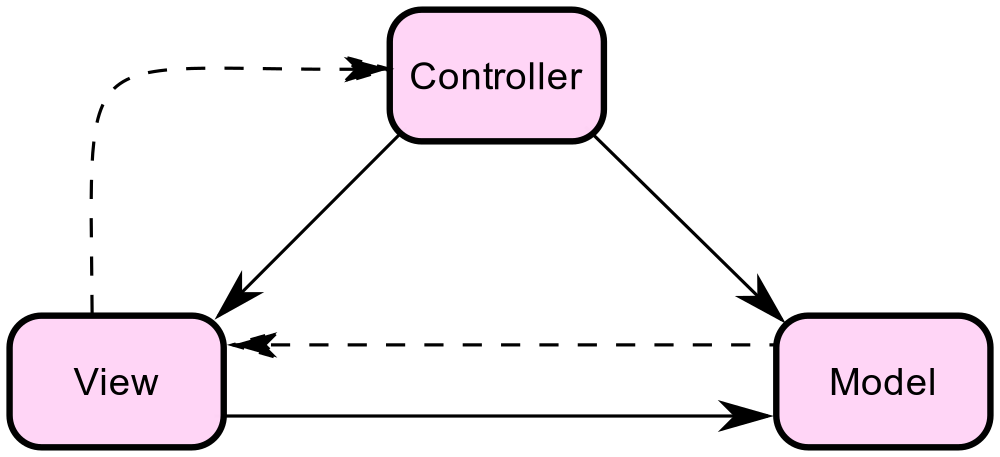
\includegraphics[scale=0.3]{images/MVC.png}
    \caption{Rappresentazione grafica del pattern MVC.}
\end{figure}

Ho scelto di usare il pattern MVC in quanto si integra perfettamente con l'architettura client-server a 3 tier caratteristica dei sistemi distribuiti che offrono servizi web. È quindi possibile assegnare ad ogni categoria di componenti del pattern MVC un tier diverso che insieme agli altri andrà a completare il sistema distribuito. La piattaforma Rius.Co. eredita quindi tutti i vantaggi caratteristici dei sistemi distribuiti e ne guadagna perciò in termini di semplicità di gestione, prestazioni e scalabilità verticale ed orizzontale \cite{3Tier}. Ulteriormente, per rendere più efficiente dal punto di vista economico e computazionale il sistema distribuito ritengo che sia necessario affidarne l'hosting e la gestione a Google tramite i numerosi servizi cloud che offre. I server che compongono il sistema distribuito saranno quindi virtuali e faranno parte di una rete altrettanto virtuale inserita nel cloud di Google.  
\medskip

Per rendere la piattaforma versatile, oltre al sito web, ho deciso di includere anche un'API (Application Programming Interface), ovvero un'ulteriore interfaccia che permette di eseguire le stesse azioni del sito web ma tramite richieste HTTPS inviate da terminale o tramite codice \cite{API}. Ho inserito la creazione di un'API nel progetto principalmente per rendere più veloce il successivo sviluppo dell'applicazione mobile che consisterebbe quindi in una semplice interfaccia grafica che dialoga direttamente con l'API. In questo caso l'API sarà contenuta in un'API server raggiungibile dall'esterno; il sito web rispetterà la stessa logica e sarà quindi contenuto in un Web server. Questi due server rappresentano perciò le View del pattern MVC. Per quanto riguarda invece i Model essi sono rappresentati dal data server che contiene tutti i dati relativi alla piattaforma. Il compito più importante del data server è gestire il database che in questo caso avrà SQLite3 come DBMS e sarà creato e manutenuto attraverso la tecnologia Microsoft Entity Framework Core. A completare l'architettura a 3 tier abbiamo quindi l'Application server che conterrà i Controller nei quali verrà definito il comportamento e la logica della Web Application. 
\medskip

Per rendere funzionante un sistema distribuito basato sull'architettura client-server a 3 tier è però necessario che i tier comunichino efficientemente tra loro, per fare ciò verranno quindi aperti dei Socket interni alla rete privata dove saranno collocati tutti i server. In questo modo le comunicazioni tra i server rimarranno private e soprattutto locali in quanto non usciranno mai dalla rete LAN. Gli utenti invece invieranno i dati al Web server e all'API server tramite il protocollo HTTPS che garantisce la sicurezza per la comunicazione HTTP. 
\medskip

Infine, scaricando la repository di GitHub \href{https://github.com/MauroPello/elaborato}{disponibile qui} \cite{GitHub} è possibile visualizzare il codice della prima versione già funzionante della Web Application sulla quale si baserà l'azienda.  